% FiLMVIB --- two-page research summary.   Build:  cd paper && pdflatex summary.tex  (x2)
%
% Provenance rule, identical to final.tex: every value below is either (a) measured under our own
% evaluation protocol or (b) reported by a cited publication, with the arXiv identifier given in the
% row. Nothing is estimated or extrapolated.  All numbers are transcribed from paper/final.tex,
% which names the source runs/*.json for each table.
%
% Dependencies are deliberately minimal: geometry, amsmath, amssymb, booktabs, xcolor, graphicx,
% tikz.  pgfplots is NOT used (it is absent on the target machines and previously broke the build) --
% every chart here is drawn in raw TikZ.  lmodern/microtype are loaded only if present.
% Figures degrade to labelled placeholder boxes when absent, so the document always compiles.
%
% LAYOUT NOTES:
%  - body is \footnotesize; captions and tables are \scriptsize; the two schematics are
%    \fitw-wrapped so they shrink rather than overflow.
%  - tables are plain centred boxes, not floats, so placement is deterministic and no full-width
%    float can collide with the title block.
%  - every tabular is sized to stay inside the column width; the wide ones use explicit p{} widths.

\documentclass[10pt,twocolumn,a4paper]{article}
\usepackage[a4paper,left=0.95cm,right=0.95cm,top=0.7cm,bottom=0.7cm,columnsep=4mm]{geometry}
\usepackage{amsmath,amssymb}
\usepackage{booktabs}
\usepackage{xcolor}
\usepackage{graphicx}
\usepackage{tikz}
\usetikzlibrary{positioning,arrows.meta,calc}
\IfFileExists{lmodern.sty}{\usepackage{lmodern}}{}
% expansion=false: font expansion needs scalable fonts, and a TeX install without lmodern falls
% back to bitmap Computer Modern, where microtype aborts the build. Protrusion works either way.
\IfFileExists{microtype.sty}{\usepackage[protrusion=true,expansion=false]{microtype}}{}

\graphicspath{{figures/}}
\definecolor{frz}{RGB}{40,95,175}     % frozen  (blue)
\definecolor{trn}{RGB}{210,120,20}    % trained (orange)
\definecolor{hdr}{RGB}{25,60,115}

\pagestyle{empty}
\setlength{\parindent}{0pt}
\setlength{\parskip}{0.5pt}
\setlength{\tabcolsep}{2.6pt}
\renewcommand{\arraystretch}{0.92}
\setlength{\abovedisplayskip}{2pt}
\setlength{\belowdisplayskip}{2pt}
\setlength{\abovedisplayshortskip}{0.5pt}
\setlength{\belowdisplayshortskip}{0.5pt}
\setlength{\textfloatsep}{2pt}

% Compact section headings, kernel-only (no titlesec dependency).
\makeatletter
\renewcommand\section{\@startsection{section}{1}{\z@}%
  {1.0ex \@plus .2ex \@minus .1ex}{0.25ex \@plus .05ex}%
  {\normalfont\small\bfseries\color{hdr}}}
\renewcommand\subsection{\@startsection{subsection}{2}{\z@}%
  {0.6ex \@plus .15ex \@minus .1ex}{0.15ex}%
  {\normalfont\small\bfseries\color{hdr}}}
\makeatother

% Tight itemize.
\newenvironment{tl}%
  {\begin{list}{$\bullet$}{\leftmargin=1.2em\itemindent=0pt\topsep=0.5pt\parsep=0pt
   \itemsep=0.4pt\labelwidth=0.85em\labelsep=0.35em}}%
  {\end{list}}

% Figure slot that degrades to a labelled box if the file is missing.
\newcommand{\figslot}[2]{\IfFileExists{figures/#1}%
  {\includegraphics[width=#2]{figures/#1}}%
  {\fbox{\parbox[c][1.8cm][c]{#2}{\centering\tiny\ttfamily\detokenize{figures/#1}}}}}

% Caption without the float machinery, so placement is exactly where it is written.
\newcommand{\cptn}[2]{\par\vspace{0.5pt}{\scriptsize\textbf{#1}~#2\par}\vspace{0.5pt}}

% Centring without the vertical padding that the center environment adds around every table.
\newenvironment{ctr}{\par\vspace{0.5pt}\begingroup\centering}{\par\endgroup\vspace{0pt}}

% Shrink-to-fit only if too wide; never enlarge. Keeps diagrams inside the text block whatever
% the installed font metrics do to their natural width.
\newcommand{\fitw}[2]{\resizebox{\ifdim\width>#1 #1\else\width\fi}{!}{#2}}

% ---- raw-TikZ horizontal bar (no pgfplots) -------------------------------------------------
% \hbarrow{baseline y}{bar length in cm}{fill colour}{row label}{value label}
% (named \hbarrow, not \hbar: amssymb already defines \hbar as the Planck constant)
\newcommand{\hbarrow}[5]{%
  \fill[#3!28,draw=#3!75!black,line width=0.3pt] (0,#1) rectangle (#2,#1+0.26);
  \node[anchor=east,font=\tiny] at (-0.08,#1+0.13) {#4};
  \node[anchor=west,font=\tiny] at (#2+0.08,#1+0.13) {#5};}

\begin{document}

\twocolumn[{%
\begin{center}
{\LARGE\bfseries\color{hdr} Making Frozen Audio--Visual LLMs Listen}\\[2pt]
{\normalsize Audio grounding via tiny adapters, anchored preference optimisation, and honest evaluation}\\[4pt]
{\small \textbf{Souleiman Sbai}}\ \ {\footnotesize---\ Research internship, final report\ \ $\cdot$\ \
Host lab: AIST CVRT\ \ $\cdot$\ \ Supervisor: Qiu Yue}\\[1pt]
{\footnotesize \texttt{souleiman.sbai@polytechnique.edu} \quad$\cdot$\quad \texttt{+33 6 20 94 64 63}}
\end{center}
\vspace{-1pt}
\begin{center}
\begin{minipage}{0.95\textwidth}\footnotesize
\textbf{Abstract.}\;
Audio--visual LLMs often answer sound questions from visual evidence: muting Qwen3-Omni's audio
leaves its answers unchanged, driving accuracy from $95.1\%$ to $0.0\%$. We attach a variational
bottleneck to each modality stream ($<\!0.5\%$ of parameters, identity at init) and train it with an
anchored preference objective on constructed audio--visual conflicts. Standard DPO on these pairs
collapses to a constant response ($0.95\!\to\!0.10$); two constraints --- a chosen-answer anchor and a
KL tether to the base model --- remove that optimum. On AVHBench ($n\!=\!5302$) the adapter gains
$+5.1$ points, and a query-conditioned (FiLM) variant $+5.8$ ($p<10^{-4}$), with hallucination
resistance preserved and no significant cost on MMAU or Video-MME. Both variants raise audio
dependence $3.3$--$3.6\times$, but only FiLM also increases attention to the evidence
($5.4\%\!\to\!7.4\%$). The gain tracks what the backbone already encodes --- $+5.8$ on Qwen3-Omni,
$+0.1$ on Qwen2.5-Omni, $-2.3$ on VideoLLaMA2 --- and on temporal alignment, where the backbone is at
chance ($0.495$), no adapter helps.
\end{minipage}
\end{center}

% ============================ FIGURE 1 (full width, in the header block) ====================
\begin{ctr}
\fitw{\textwidth}{%
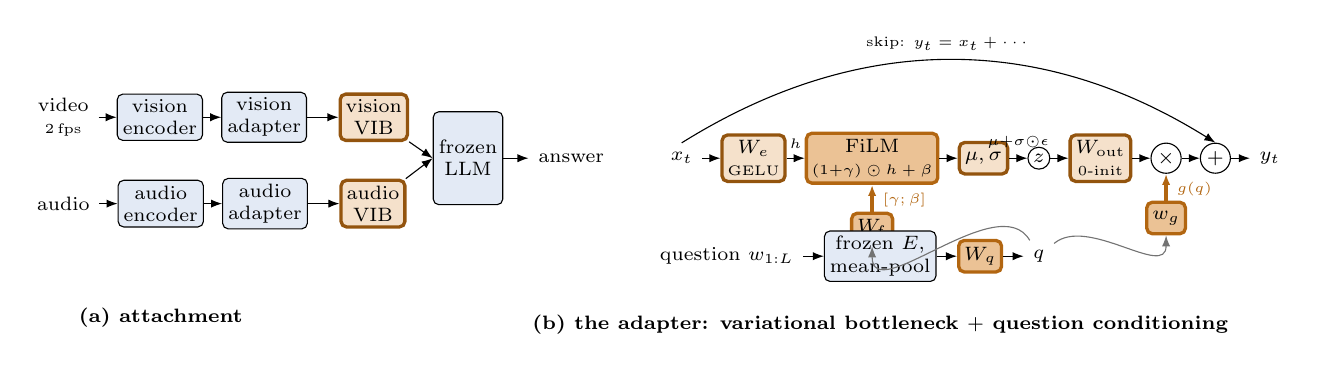
\begin{tikzpicture}[font=\scriptsize,>={Latex[length=1.4mm]},node distance=1.3mm and 2.3mm,
  trn/.style={draw,very thick,rounded corners=2pt,fill=trn!22,draw=trn!70!black,
              minimum height=4.0mm,inner sep=2pt,align=center},
  new/.style={draw,very thick,rounded corners=2pt,fill=trn!45,draw=trn!85!black,
              minimum height=4.0mm,inner sep=2pt,align=center},
  frzs/.style={draw,rounded corners=2pt,fill=frz!13,minimum height=4.0mm,inner sep=2pt,align=center},
  op/.style={draw,circle,inner sep=1pt},
  io/.style={align=center}]

  % ---------- (a) where the module attaches ----------
  \node[io] (vin) {video\\{\tiny 2\,fps}};
  \node[frzs,right=of vin] (venc) {vision\\encoder};
  \node[frzs,right=of venc] (vproj) {vision\\adapter};
  \node[io,below=5.2mm of vin] (ain) {audio};
  \node[frzs,right=of ain] (aenc) {audio\\encoder};
  \node[frzs,right=of aenc] (aproj) {audio\\adapter};
  \node[trn,right=4mm of vproj] (vvib) {vision\\VIB};
  \node[trn,right=4mm of aproj] (avib) {audio\\VIB};
  \node[frzs,right=3mm of vvib,yshift=-5.2mm,minimum height=11.8mm] (llm) {frozen\\LLM};
  \node[io,right=3.2mm of llm] (ans) {answer};
  \draw[->] (vin)--(venc); \draw[->] (venc)--(vproj); \draw[->] (vproj)--(vvib); \draw[->] (vvib)--(llm.west);
  \draw[->] (ain)--(aenc); \draw[->] (aenc)--(aproj); \draw[->] (aproj)--(avib); \draw[->] (avib)--(llm.west);
  \draw[->] (llm)--(ans);
  \node[anchor=north,font=\scriptsize\bfseries] at ([yshift=-9mm]aenc.south) {(a) attachment};

  % ---------- (b) module internals ----------
  \node[io,right=6mm of ans] (x) {$x_t$};
  \node[trn,right=of x] (enc) {$W_e$\\{\tiny GELU}};
  \node[new,right=of enc] (film) {FiLM\\{\tiny $(1{+}\gamma)\odot h+\beta$}};
  \node[trn,right=of film] (ms) {$\mu,\sigma$};
  \node[op,right=of ms] (z) {$z$};
  \node[trn,right=of z] (wo) {$W_{\text{out}}$\\{\tiny 0-init}};
  \node[op,right=of wo] (mult) {$\times$};
  \node[op,right=of mult] (add) {$+$};
  \node[io,right=2.4mm of add] (y) {$y_t$};
  \draw[->] (x)--(enc); \draw[->] (enc)--node[above]{\tiny $h$}(film);
  \draw[->] (film)--(ms); \draw[->] (ms)--node[above]{\tiny $\mu{+}\sigma{\odot}\epsilon$}(z);
  \draw[->] (z)--(wo); \draw[->] (wo)--(mult); \draw[->] (mult)--(add); \draw[->] (add)--(y);
  \draw[->] (x.north) to[out=32,in=148] node[above,pos=0.5]{\tiny skip: $y_t=x_t+\cdots$} (add.north);
  % --- question path: FiLM/gate heads on their own row, question row clear below them ---
  \node[new,below=3.4mm of film] (wf) {$W_{\!f}$};
  \node[new,below=3.4mm of mult] (wg) {$w_g$};
  \draw[->,trn!85!black,very thick] (wf)--node[right,pos=0.42]{\tiny $[\gamma;\beta]$}(film);
  \draw[->,trn!85!black,very thick] (wg)--node[right,pos=0.42]{\tiny $g(q)$}(mult);
  \node[io,below=10.5mm of x,anchor=west,xshift=-4mm] (w) {question $w_{1:L}$};
  \node[frzs,right=2.6mm of w] (embed) {frozen $E$,\\mean-pool};
  \node[new,right=2.6mm of embed] (wq) {$W_q$};
  \node[io,right=2.6mm of wq] (qv) {$q$};
  \draw[->] (w)--(embed); \draw[->] (embed)--(wq); \draw[->] (wq)--(qv);
  \draw[->,black!55] (qv) to[out=120,in=-90] (wf);
  \draw[->,black!55] (qv) to[out=40,in=-90] (wg);
  \node[anchor=north,font=\scriptsize\bfseries] at ([yshift=-3mm]embed.south)
        {(b) the adapter: variational bottleneck $+$ question conditioning};
\end{tikzpicture}}
\end{ctr}
\cptn{Figure 1.}{\textbf{(a)} One bottleneck per modality, after the frozen projection adapter (LLM
embedding space); blue $=$ frozen, orange $=$ trained. \textbf{(b)} Internals ---
$z=\mu(x)+\sigma(x)\odot\epsilon$, $y=x+W_{\text{out}}z$, $W_{\text{out}}\!\stackrel{\text{init}}{=}\!0$
(\S2.1) --- with the FiLM path (darker) reading a pooled, frozen question embedding and emitting a
per-feature scale/shift $[\gamma;\beta]$ and gate $g(q)$; $\gamma,\beta$ are FiLM's parameters (Perez
et al., 2018), not the DPO temperature $\beta$ or bottleneck rate $\beta_{kl}$.}
}]

\footnotesize

% ================================================================================================
\section{The problem: sound answered from sight}

Audio--visual LLMs tokenize each modality (audio $\sim$25/s; video at 2\,fps here) and answer over the
mixed sequence --- audio consistently loses to vision. \textbf{AVHBench} (Sung-Bin et al., ICLR'25),
\textbf{CMM} (Leng et al., 2024) and \textbf{Wen et al.} (2026, a \emph{Clever Hans} effect) all report
this bias; Wen et al.'s interventions on \emph{our} backbone, Qwen3-Omni, are decisive (accuracy \%):

\begin{ctr}\scriptsize
\begin{tabular}{@{}l cc l@{}}
\toprule
probe & original & intervened & intervention \\
\midrule
audio existence   & 95.1  & \textcolor{red!70!black}{\textbf{0.0}}  & \emph{Mute}: silence the track \\
temporal sync     & 100.0 & \textcolor{red!70!black}{\textbf{1.4}}  & \emph{Shift}: audio moved $\pm2$\,s \\
sound consistency & 75.4  & \textcolor{red!70!black}{\textbf{37.3}} & \emph{Swap}: another clip's audio \\
\bottomrule
\end{tabular}
\end{ctr}
\cptn{Table 1.}{Reported, arXiv:2605.16403 Tab.~1. Under muting accuracy falls to \emph{zero}, not
chance: answers stay consistent with the \emph{video}.}

Mitigations (contrastive decoding, modality-decoupled DPO, full re-alignment) all modify or bypass the
backbone. \textbf{Our question: can a frozen backbone's audio grounding be improved by a
parameter-efficient adapter alone?}

% ================================================================================================
\section{Method}

\subsection{A variational bottleneck per stream}
The information bottleneck (Tishby et al., 2000) seeks a compressed $Z$ retaining only what predicts
$Y$: $\max_{q(z|x)} I(Z;Y)-\beta_{kl}I(Z;X)$, both terms replaced by variational bounds (Alemi et al.,
ICLR'17), encoder trained by reparameterisation. Per modality (Fig.~1b):
\[ z=\mu(x)+\sigma(x)\odot\epsilon,\quad y=x+W_{\text{out}}z,\quad W_{\text{out}}\stackrel{\text{init}}{=}0 .\]
The two modules are $<\!0.5\%$ of backbone parameters, are the \emph{identity at initialisation}, and
bypassing them reproduces the frozen backbone bit-for-bit (the free DPO reference).

\subsection{Training data: constructed conflicts}
Substituting a clip's audio track yields an instance where the visible and audible events disagree (a
flute in view, a train horn heard); preferring the audio-consistent answer is only possible by using
the audio.

\subsection{Why standard DPO fails}
With $c,r$ the log-probabilities of the chosen (heard) and rejected (seen) answer ($p=$ adapter on,
$r=$ bypassed):
\[ \mathcal L_{\text{DPO}}=-\log\sigma\big(\beta[(c_p-c_r)-(r_p-r_r)]\big),\quad \beta=0.1 , \]
where $\sigma$ is the sigmoid, \emph{not} the encoder's $\sigma(x)$. This constrains only the
\emph{margin}, so it is minimised even as both probabilities fall provided the rejected one falls
faster --- the displaced mass lands on an unconstrained third response (\emph{likelihood
displacement}). The model converges to answering ``no'' everywhere ($0.95\!\to\!0.10$) while \emph{maximising}
hallucination resistance: that score alone is not a sufficient signal.

\subsection{Anchored objective}
\begin{align*}
\mathcal L =\ &\underbrace{-\log\sigma\big(\beta[(c_p{-}c_r){-}(r_p{-}r_r)]\big)}_{\text{\scriptsize \textbf{engine}: prefer the heard answer}}\\[1pt]
 &+\ \lambda_a\underbrace{\big({-}\log\sigma(\beta(c_p{-}c_r){-}\delta)\big)}_{\text{\scriptsize\color{trn}\textbf{rail 1}: chosen $\ge$ base $\Rightarrow$ PA}}\\[1pt]
 &+\ \lambda_{kl}\underbrace{\mathrm{KL}(p_{\text{base}}\|p_\theta)}_{\text{\scriptsize\color{trn}\textbf{rail 2}: normal inputs $\Rightarrow$ HR}}
   \ +\ \beta_{kl}\,\mathrm{KL}_{\text{VIB}}
\end{align*}
Rail 1 (mDPO-style) forbids the chosen response from losing probability against the base model; rail
2 tethers ordinary, non-substituted inputs to it. The uniform-``no'' solution violates both, so the
preference term can only shrink by \emph{using the audio}.

% ================================================================================================
\section{Evaluation protocol}

\textbf{AVHBench} ($n\!=\!5302$, 2{,}136 videos): A$\to$V $1{,}136$, V$\to$A $2{,}290$, A--V Matching
$1{,}876$; balanced, so chance is $50\%$. V$\to$A (a queried sound audible) is our primary measure.
\textbf{CMM} ($1{,}200\times2=2{,}400$) reports PA/HR jointly: ``no'' always gives $\text{HR}=1.0$,
$\text{PA}=0$.

\begin{tl}\scriptsize
\item \textbf{Frame rate}: 2\,fps for Qwen3-Omni (1\,fps, 7B backbones), fixed for selection and
evaluation alike; below 2\,fps Qwen3-Omni develops a yes-bias.
\item \textbf{Prompt sensitivity is large}: the answer-format suffix alone moved one score by $+11$
points (V$\to$A, $69.0\!\to\!80.3$) at identical weights, so prompts, suffix and decoding are fixed
and logged.
\item \textbf{Checkpoint selection} on a validation half, reported on the disjoint remainder --- the
first-selected checkpoint did not survive this.
\item \textbf{Paired significance}: identical items for both models; McNemar with bootstrap CIs.
\textbf{Contamination}: training$\,\cap\,$benchmark clips $=\emptyset$, verified by script.
\end{tl}

% ================================================================================================
\section{Results}

\begin{ctr}\scriptsize
\setlength{\tabcolsep}{2.2pt}
\begin{tabular}{@{}l cccc ccc@{}}
\toprule
& \multicolumn{4}{c}{AVHBench ($n{=}5302$)} & \multicolumn{3}{c}{CMM ($n{=}2400$)} \\
\cmidrule(lr){2-5}\cmidrule(lr){6-8}
 & $A\!\to\!V$ & $V\!\to\!A$ & AV-m & \textbf{all} & PA & HR & all \\
\midrule
Gemini {\tiny(closed)} & 0.850 & 0.747 & 0.603 & 0.718 & 0.907 & 0.628 & 0.768 \\
GPT-4o {\tiny(closed)} & 0.846 & 0.510 & 0.501 & 0.579 & 0.359 & 0.892 & 0.626 \\
\midrule
frozen base                        & \textbf{0.838} & 0.812 & 0.653 & 0.761 & \textbf{0.900} & 0.733 & 0.816 \\
$+$ cross-attn {\tiny(st.\ 60)}    & \textbf{0.850} & 0.805 & 0.696 & 0.776 & \multicolumn{3}{c}{\emph{CMM running}} \\
$+$ LoRA $r{=}16$ {\tiny(st.\ 90)} & 0.828 & 0.835 & 0.709 & 0.789 & 0.896 & 0.724 & 0.810 \\
$+$ swap-DPO {\tiny(st.\ 60)}      & 0.837 & \textbf{0.838} & 0.766 & 0.812 & 0.890 & 0.743 & 0.816 \\
$+$ \textbf{FiLM} {\tiny(st.\ 160)}& 0.822 & 0.827 & \textbf{0.808} & \textbf{0.819} & 0.894 & \textbf{0.746} & \textbf{0.820} \\
\bottomrule
\end{tabular}
\end{ctr}
\cptn{Table 3.}{One protocol; both adapters gain $+5.1$/$+5.8$ points, preserving capability (HR up,
PA down $\le1$), concentrated in A--V Matching ($0.653\!\to\!0.808$, $+15.5$). GPT-4o's
$\text{HR}\,0.892$/PA $0.359$ is \S2.3's degenerate solution, deployed.}

\begin{ctr}\scriptsize
\begin{tabular}{@{}l c c l@{}}
\toprule
comparison (held-out) & $b/c$ & $\Delta$ [95\% CI] & verdict \\
\midrule
base $\to$ swap-DPO & 152/411 & $+5.2$ [{+}4.3, {+}6.1] & real ($p<10^{-4}$) \\
base $\to$ FiLM     & 253/532 & $+5.6$ [{+}4.5, {+}6.7] & real ($p<10^{-4}$) \\
DPO $\to$ FiLM      & 204/224 & $+0.4$ [{-}0.4, {+}1.2] & tie \\
\bottomrule
\end{tabular}
\end{ctr}
\cptn{Table 4.}{Only discordant pairs inform ($b$: baseline alone, $c$: adapted alone); $411$ vs
$152$ rejects a fair-coin null. FiLM beats swap-DPO on A--V Matching by $+3.7$ ($p<10^{-4}$).
\emph{Single seed}: item sampling only.}

\subsection{Capability controls}

\begin{ctr}\scriptsize
\begin{tabular}{@{}l cccc c cc@{}}
\toprule
& \multicolumn{4}{c}{MMAU ($n{=}1000$)} & & \multicolumn{2}{c}{Video-MME ($n{=}900$)} \\
\cmidrule(lr){2-5}\cmidrule(lr){7-8}
Qwen3-Omni & Snd & Mus & Sph & Avg & & acc & $\Delta$ \\
\midrule
frozen base  & \textbf{80.2} & \textbf{75.4} & \textbf{68.5} & \textbf{74.7} & & \textbf{0.842} & --- \\
$+$ swap-DPO & 78.4 & 75.1 & 67.0 & 73.5 & & 0.828 & $-1.4$ \\
$+$ FiLM     & 79.6 & 73.1 & 66.4 & 73.0 & & 0.837 & $-0.6$ \\
\bottomrule
\end{tabular}
\end{ctr}
\cptn{Table 5.}{Two OOD controls, one pinned harness; MMAU parse $0.94$, Video-MME is the
\textbf{short} subset \textbf{without} subtitles. The $95\%$ intervals ($\pm2.8$, $\pm2.4$) make every
difference non-significant --- but each is \emph{negative}, reported as such. FiLM preserves
capability better than swap-DPO: learning which modality to trust does not transfer to audio
understanding at large.}

% ================================================================================================
\section{Mechanism: what the adapter changes}

Accuracy alone cannot distinguish two adapters with the same gain. Three probes do: \textbf{(i)}
attention share on audio/video tokens at the answer position (comparable \emph{within} a model
only); \textbf{(ii)} re-scoring the gold answer under substituted audio, since a model that ignores
audio shifts by $\approx0$ (Fig.~3); \textbf{(iii)} reading the trained FiLM checkpoint directly.

\begin{ctr}
\fitw{\linewidth}{%
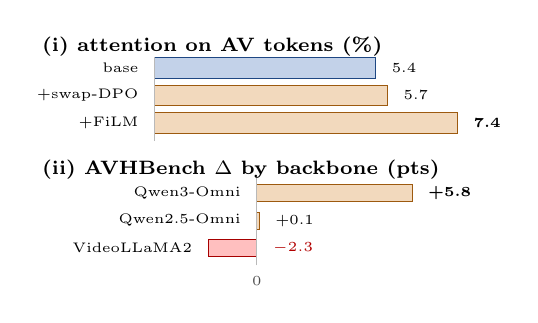
\begin{tikzpicture}[font=\scriptsize]
% ---- panel (i): attention share, %  (scale 0.52 cm per point) ----
\node[anchor=west,font=\scriptsize\bfseries] at (-1.55,1.10) {(i) attention on AV tokens (\%)};
\hbarrow{0.70}{2.81}{frz}{base}{5.4}
\hbarrow{0.35}{2.96}{trn}{+swap-DPO}{5.7}
\hbarrow{0.00}{3.85}{trn}{+FiLM}{\textbf{7.4}}
\draw[gray!55,line width=0.3pt] (0,-0.10) -- (0,0.97);
% ---- panel (ii): cross-backbone delta (scale 0.34 cm per point, zero at x=1.30) ----
\node[anchor=west,font=\scriptsize\bfseries] at (-1.55,-0.46) {(ii) AVHBench $\Delta$ by backbone (pts)};
\fill[trn!28,draw=trn!75!black,line width=0.3pt] (1.30,-0.87) rectangle (3.27,-0.65);
\node[anchor=east,font=\tiny] at (1.22,-0.76) {Qwen3-Omni};
\node[anchor=west,font=\tiny] at (3.35,-0.76) {\textbf{+5.8}};
\fill[trn!28,draw=trn!75!black,line width=0.3pt] (1.30,-1.22) rectangle (1.33,-1.00);
\node[anchor=east,font=\tiny] at (1.22,-1.11) {Qwen2.5-Omni};
\node[anchor=west,font=\tiny] at (1.41,-1.11) {+0.1};
\fill[red!25,draw=red!65!black,line width=0.3pt] (0.68,-1.57) rectangle (1.30,-1.35);
\node[anchor=east,font=\tiny] at (0.60,-1.46) {VideoLLaMA2};
\node[anchor=west,font=\tiny] at (1.38,-1.46) {\textcolor{red!70!black}{$-2.3$}};
\draw[gray!55,line width=0.3pt] (1.30,-1.68) -- (1.30,-0.57);
\node[anchor=north,font=\tiny,text=gray!60!black] at (1.30,-1.70) {0};
\end{tikzpicture}}
\end{ctr}
\cptn{Figure 2.}{Bar lengths proportional to the data. (i) Qwen3-Omni: $5.4\%\!\to\!5.7\%$ for
swap-DPO (unchanged) versus $5.4\%\!\to\!7.4\%$ for FiLM ($38\%$ relative); Qwen2.5-Omni
$7.9\%\!\to\!8.1\%$. (ii) Identical data, objective and selection per backbone.}

\begin{ctr}
\figslot{ll_shift.png}{0.90\linewidth}
\end{ctr}
\cptn{Figure 3.}{Log-likelihood of the gold answer, true (teal) vs substituted (magenta) audio; KDE
over $40$ AVE clips, dashed $=$ means. Shifts: base $-0.515$, $+$swap-DPO $-1.698$, $+$FiLM
$-\mathbf{1.848}$ --- a $3.3$--$3.6\times$ rise.}

\textbf{Reading.} Comparable gains, two mechanisms: swap-DPO raises audio dependence \emph{without}
attending more to it (re-encoding); FiLM raises both. Probes agree: $\|W_{\text{out}}\|/\|W_e\|\approx1.0$
(rotates, not amplifies), gate $g(q)$ \textbf{never $<0.4$} (modulation, not routing), modulation
$\approx4.5\times$ stronger on vision --- the query mostly re-weights it.

% ================================================================================================
\section{Generalisation, and the bound on the method}

\begin{ctr}\scriptsize
\begin{tabular}{@{}l cc c l@{}}
\toprule
backbone & base & $+$adapter & $\Delta$ & attention on AV \\
\midrule
Qwen3-Omni (30B)   & 0.761 & \textbf{0.819} & $+5.8$ & $5.4\%\!\to\!7.4\%$ \\
Qwen2.5-Omni (7B)  & 0.729 & 0.730 & $+0.1$ & $7.9\%\!\to\!8.1\%$ \\
VideoLLaMA2 (7B)   & 0.707 & 0.684 & \textcolor{red!70!black}{$-2.3$} & audio added post hoc \\
MiniCPM-O 2.6 (8B) & 0.744 & \emph{training} & --- & --- \\
\bottomrule
\end{tabular}
\end{ctr}
\cptn{Table 6.}{AVHBench overall, $n{=}5302$: gain tracks audio \emph{already present} --- an adapter
makes it \emph{usable}, but cannot supply competence the backbone lacks.}

\textbf{Harness sensitivity, quantified.} On MiniCPM-O 2.6 (identical weights/benchmark), our harness
gives AVHBench $\mathbf{0.744}$ against the published $0.693$ (arXiv:2603.03192) --- $5.1$ points
apart from prompt/frame-rate choices, so we compare relative gains within one protocol only. Its CMM
$\text{HR}\,0.578$ (PA $0.897$) vs $0.733$ for Qwen3-Omni: weaker grounding, more headroom.

\begin{ctr}\scriptsize
\setlength{\tabcolsep}{2.2pt}
\begin{tabular}{@{}l l c c l@{}}
\toprule
backbone & method & base $\to$ trained & $\Delta$ & trains \\
\midrule
MiniCPM-O 2.6 & MoD-DPO++ {\tiny(rep.)} & $0.693\!\to\!0.745$ & $+5.2$ & \textcolor{red!70!black}{full LLM} \\
Qwen2.5-Omni  & MoD-DPO++ {\tiny(rep.)} & $0.708\!\to\!0.796$ & $+8.8$ & \textcolor{red!70!black}{full LLM} \\
Qwen2.5-Omni  & MAD {\tiny(rep.)}       & $0.769\!\to\!0.816$ & $+4.7$ & \textcolor{frz}{decode-time} \\
\midrule
Qwen3-Omni    & \textbf{FiLM (ours)}    & $0.761\!\to\!0.819$ & \textbf{+5.8} & \textcolor{trn}{\textbf{0.5\% adapter}} \\
\bottomrule
\end{tabular}
\end{ctr}
\cptn{Table 7.}{Reported rows: arXiv:2603.03192, arXiv:2601.21181, each on \emph{their}
backbone/harness --- deltas only. Ours sits between full fine-tuning ($+8.8$) and decode-time
($+4.7$), updating $<0.5\%$ of parameters, reversibly; on A--V Matching, $+15.5$ matches MoD-DPO's
$+15.0$.}

% ================================================================================================
\section{Temporal alignment: a negative result that explains the rest}

The same objective applies to a different intervention --- displace the audio by
$\Delta\in\pm\{0.5,1,2\}$s and prefer the correct synchronisation judgement, rails unchanged. It
fails, instructively.

\begin{ctr}\scriptsize
\begin{tabular}{@{}l c l@{}}
\toprule
AVE-Shift (held out, balanced $\Rightarrow$ chance $0.50$) & acc & reading \\
\midrule
base --- synchronised vs shifted ($n{=}200$)     & 0.495 & at chance \\
base --- lag vs lead ($n{=}100$)                 & 0.500 & at chance \\
base --- $\pm2$\,s displacement only ($n{=}200$) & 0.495 & at chance \\
\midrule
$+$ shift-DPO {\tiny(st.\ 60)} --- sync vs shifted & 0.515 & unchanged \\
$+$ shift-DPO {\tiny(st.\ 60)} --- lag vs lead     & 0.450 & unchanged \\
\bottomrule
\end{tabular}
\end{ctr}
\cptn{Table 8.}{All differences lie inside the $\pm7$-point interval here. Row 3 restricts to
$\pm2$s --- four frames at 2\,fps, the most resolvable offset --- and the backbone is at chance there
too.}

Training on displaced data leaves accuracy at chance: \textbf{the backbone carries no usable
temporal-alignment signal, so there is nothing to unlock} --- the same pattern as audio on
VideoLLaMA2, stating the law behind this method: \emph{gain is proportional to usable-but-underused
signal}. This also reconciles our $0.495$ with Table~1's $100.0\!\to\!1.4$: always answering
``synchronised'' scores $\approx100$ on synchronised items, $\approx0$ on displaced ones, $\approx50$
overall.

As a controlled test of representability we add a shared clock feature
$\tau_t=[\sin(2\pi t/T),\cos(2\pi t/T)]$ to both streams before the bottleneck, making misalignment
representable at all ($0.5$s frame interval at 2\,fps bounds the smallest displacement). \emph{Implemented
and training, as a test of the hypothesis, not an expected improvement.}

% ================================================================================================
\section{Negative results, limitations, status}

\textbf{Six things that did not survive contact with data}: standard DPO on swap pairs collapsed to a
constant response (PA $0.95\!\to\!0.10$), motivating the two rails; GRPO on easy items gave zero
advantage on ${\sim}2/3$ of steps (unanimous rewards, no gradient); gate $g(q)$ as a router stayed
$>0.4$ throughout (modulation beats routing); a $59\%$-of-vision-rewritten claim did not survive
inspection and was withdrawn; LoRA at identical attach points reached $+2.8$ against FiLM's $+5.1$,
HR \emph{below} base (residual form matters, not capacity); and pre-adapter placement matched
accuracy but not portability (one attachment width per backbone, not per modality) --- untabulated.

\textbf{Single seed}: intervals reflect item sampling, not seed variance; a $\beta_{kl}$ sweep,
VIB-ingredient ablation and data-scaling curve are not yet measured. \textbf{In progress}: CMM for
cross-attention; MiniCPM-O adapter training; video-substitution and temporal-displacement variants,
trained but unevaluated. \textbf{Reproducibility}: four model wrappers, five benchmark runners, four
training variants, three probes, ${\approx}10$k lines, 23 job scripts, seven test suites; frame rate,
prompts and decoding pinned, selection on a disjoint validation half, per-item predictions stored for
recomputation.

% ================================================================================================
\section{Conclusion}

A zero-initialised variational adapter ($<\!0.5\%$ of parameters) improves audio grounding in a
\emph{frozen} audio--visual LLM by $+5.1$--$5.8$ AVHBench points ($p<10^{-4}$), free on capability,
backed by mechanism, not just accuracy. Its limit is equally measured: no usable signal, no adapter can
supply it --- audio on VideoLLaMA2, timing on Qwen3-Omni.

\end{document}
